\documentclass[border=10pt]{standalone}

\usepackage{tikz}
\usepackage{tikzsymbols}
\usetikzlibrary{calc,patterns,shapes.geometric}

\def\centerarc[#1](#2)(#3:#4:#5){\draw[#1] ($(#2)+({#5*cos(#3)},{#5*sin(#3)})$) arc (#3:#4:#5);}

\begin{document}
	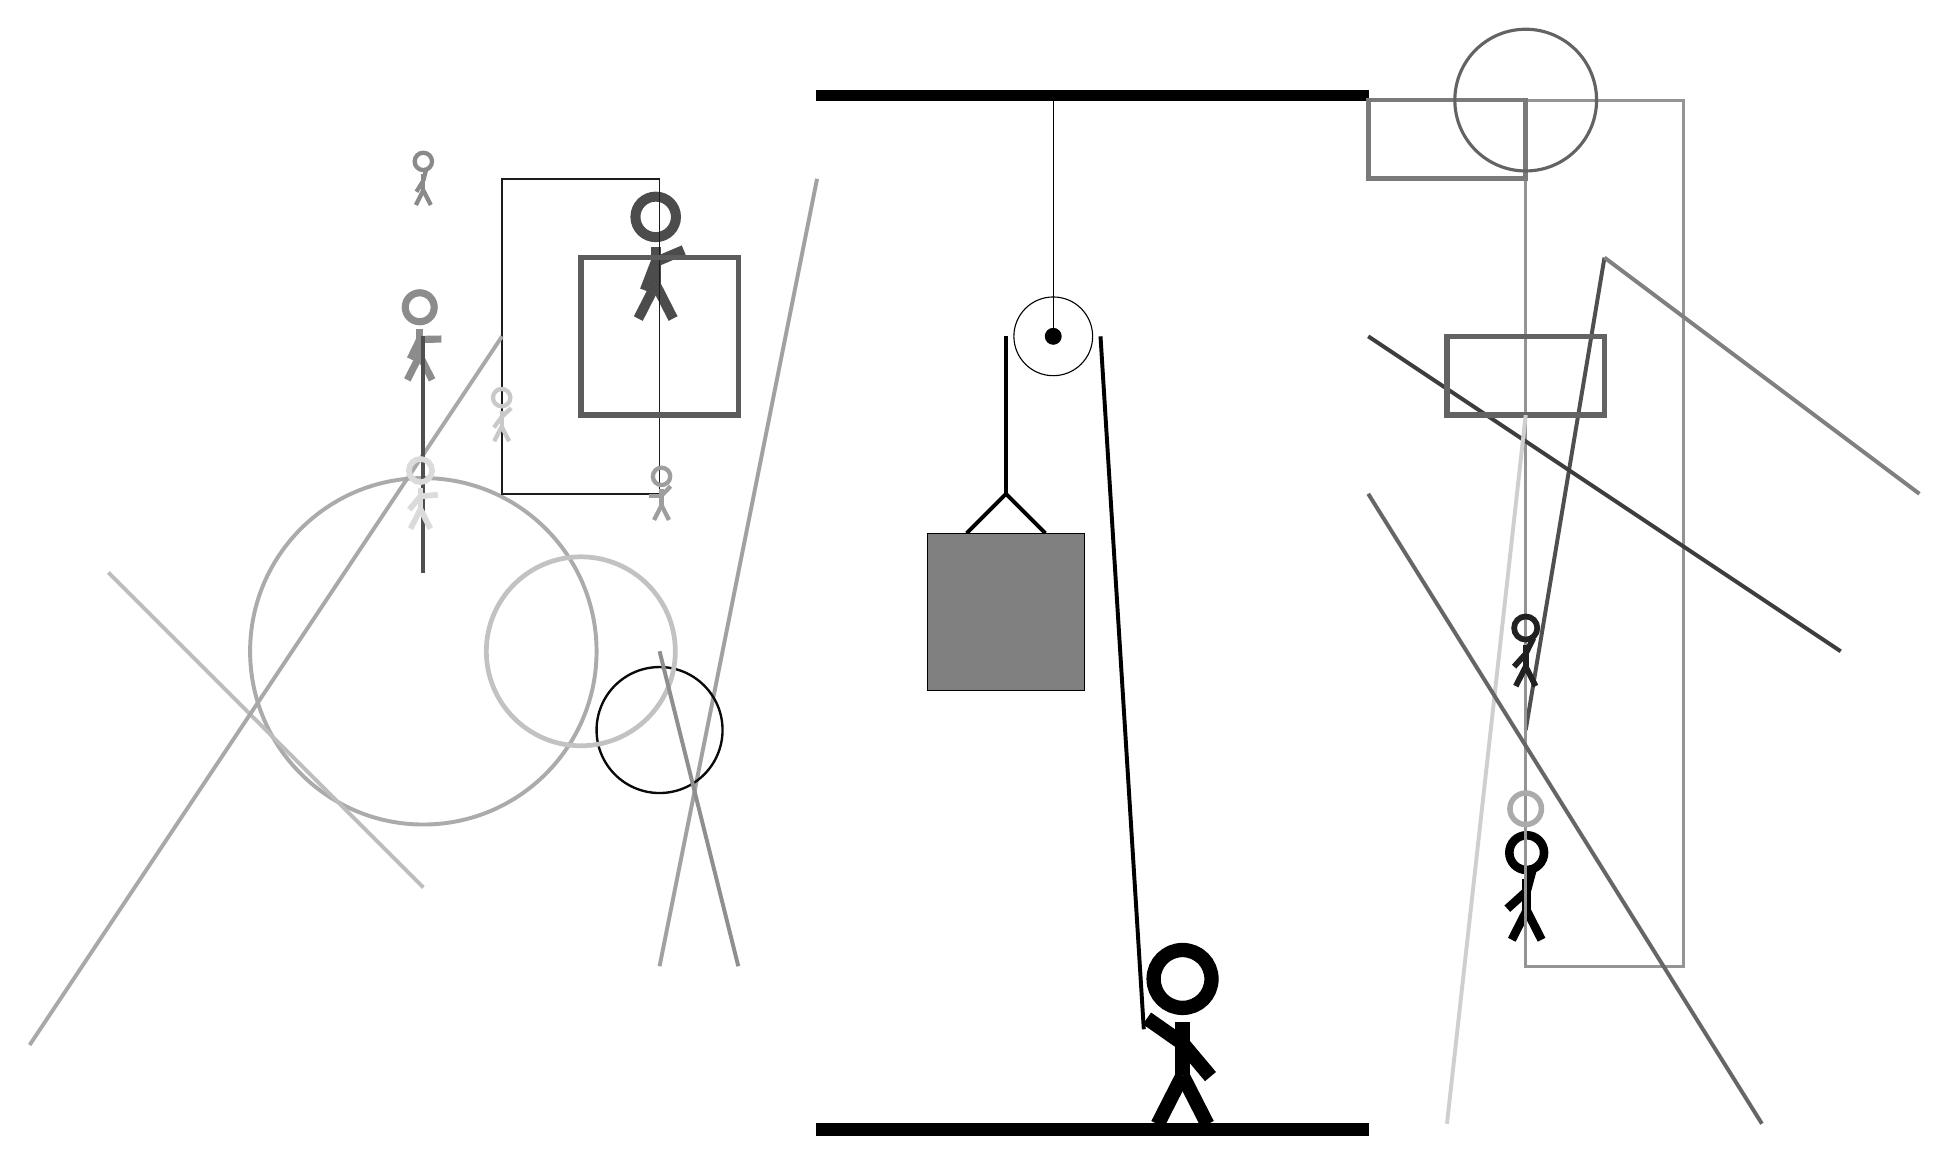
\begin{tikzpicture}
		%%%%% START %%%%%
		
		\draw[fill=black] (-2, 10) rectangle (5, 10.125);
		
		\draw (1, 7) circle (0.5);
		\draw[fill=black] (1, 7) circle (0.1);
		\draw (1, 10) -- (1, 7);
		
		\draw[line width=0.5mm] (-0.1, 4.5) -- (0.4, 5.0) -- (0.9, 4.5);
		\draw[fill=black!50] (-0.6, 4.5) rectangle (1.4, 2.5);
		
		\draw[line width=0.5mm, color=black!69](7, 2) -- (8, 8);
		
		\draw [line width=0.5mm, color=black!33](-7, 3) circle (2.2);
		\node[line width=0.4mm, color=black!100] at (7, 0) {\Strichmaxerl[6][42][75]};
		\draw[line width=0.4mm, color=black!42] (7, -1) rectangle (9, 10);
		
		\draw[line width=0.6mm, color=black!52] (5, 10) rectangle (7, 9);
		\node[line width=0.7mm, color=black!70] at (-4, 8) {\Strichmaxerl[7][69][23]};
		\draw[line width=0.5mm, color=black!26](-7, 0) -- (-11, 4);
		\draw[line width=0.2mm, color=black!89] (-4, 5) rectangle (-6, 9);
		\draw[line width=0.5mm, color=black!37](-2, 9) -- (-4, -1);
		\draw[line width=0.5mm, color=black!76](5, 7) -- (11, 3);
		\draw [line width=0.3mm, color=black!96](-4, 2) circle (0.8);
		\draw[line width=0.7mm, color=black!61] (6, 7) rectangle (8, 6);
		\node[line width=0.3mm, color=black!21] at (-6, 6) {\Strichmaxerl[3][54][43]};
		\draw[line width=0.7mm, color=black!64] (-3, 8) rectangle (-5, 6);
		\draw [line width=0.4mm, color=black!61](7, 10) circle (0.9);
		\node[line width=0.6mm, color=black!46] at (-7, 9) {\Strichmaxerl[3][58][76]};
		
		\draw[line width=0.5mm, color=black!19](7, 6) -- (6, -3);
		\draw [line width=0.6mm, color=black!24](-5, 3) circle (1.2);
		\draw [line width=0.7mm, color=black!33](7, 1) circle (0.2);
		\node[line width=0.5mm, color=black!45] at (-7, 7) {\Strichmaxerl[5][64][1]};
		\draw[line width=0.5mm, color=black!34](-6, 7) -- (-12, -2);
		\draw[line width=0.5mm, color=black!60](10, -3) -- (5, 5);
		\draw[line width=0.5mm, color=black!50](8, 8) -- (12, 5);
		\node[line width=0.6mm, color=black!38] at (-4, 5) {\Strichmaxerl[3][0][46]};
		\node[line width=0.3mm, color=black!87] at (7, 3) {\Strichmaxerl[4][48][64]};
		\draw[line width=0.5mm, color=black!69](-7, 7) -- (-7, 4);
		
		\draw[line width=0.5mm, color=black!44](-3, -1) -- (-4, 3);
		\node[line width=0.7mm, color=black!14] at (-7, 5) {\Strichmaxerl[4][50][5]};
		
		\draw[line width=0.5mm] (0.4, 7) -- (0.4, 5.0);
		\centerarc[line width=0.5mm](1, 7)(0:180:0.6);
		\draw[line width=0.5mm](1.6, 7) -- (2.15, -1.8);
		
		\node at (2.6, -1.9) {\Strichmaxerl[10][-35][-50]};
		
		\draw[fill=black] (-2, -3) rectangle (5, -3.15);
		
		%%%%% END %%%%%
	\end{tikzpicture}
\end{document}